\documentclass[letterpaper,12pt]{article}
\usepackage[utf8]{inputenc}
\usepackage{geometry}
\usepackage{amsmath}
\usepackage{float}
\usepackage{graphicx}
\usepackage{subcaption}
\usepackage{amssymb}
\usepackage{adjustbox}
\usepackage{wrapfig} %%imagen envuelta por un texto
\usepackage{xcolor}
\usepackage{fancyhdr}

\geometry{top=2.54cm, bottom=2.54cm, left=3cm, right= 3cm} 
\graphicspath{{images/}}
\renewcommand{\baselinestretch}{1.5} %%interlineadou :)
\parindent=0pt

\title{ \huge \textbf{Correlación entre carreras \\ de ingeniería y gastos estudiantiles} \\  \large Un análisis exploratorio enfocado en alumnos de la \\ Facultad de Ingeniería Eléctrica y Electrónica}
\author{Experiencia educativa "Probabilidad y Estadística" \\ cursada con la Dra. Reyna Lorena Nevero Arriola \\ Lara Xocuis Martha Denisse \\ López Castillo Haziel \\ Martínez Schleske Alan \\ Themsel Montes Guillermo Francisco \\ Facultad de Ingeniería Eléctrica y Electrónica }
\date{Martes 23 de Mayo del 2023}

\begin{document}
\maketitle
\thispagestyle{empty}

\begin{figure}[H]
    \centering
    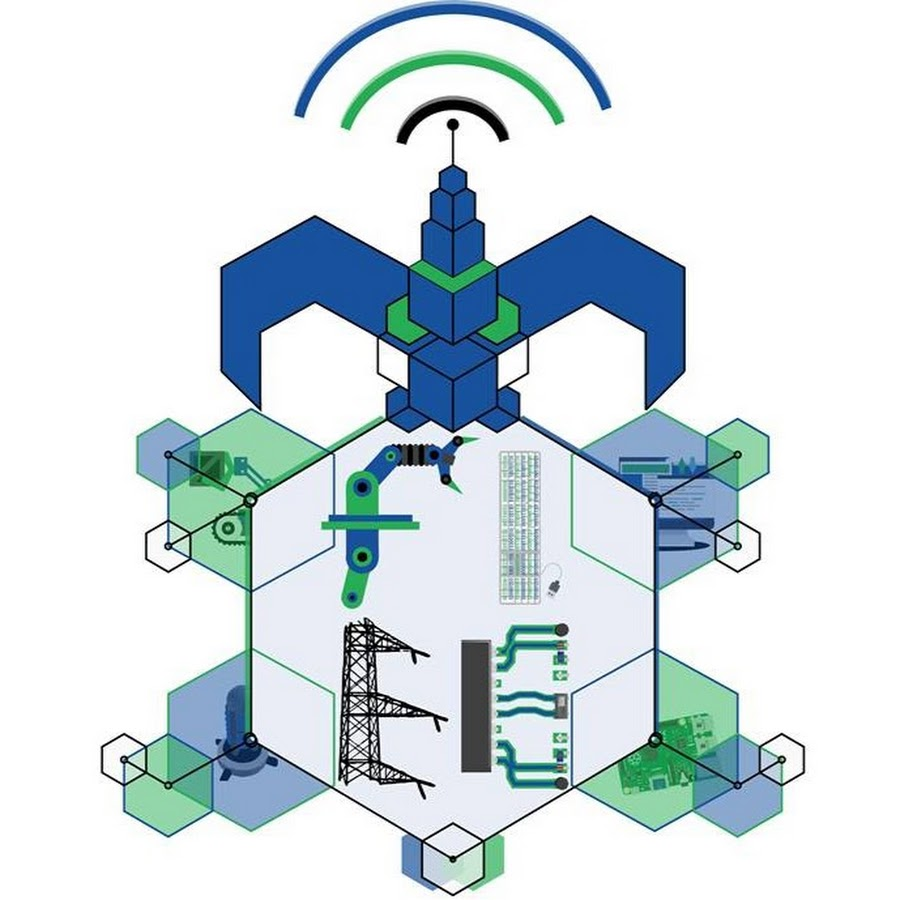
\includegraphics[width=0.4\textwidth]{images/probabilidad/logo FIEE.jpg}
\end{figure}

\newpage

\setcounter{page}{1}
\pagestyle{headings}

\newpage
%%%%%%%%%%%%%%%%%%%%%%%%%%%%%%%%%%%%%%%%%%%%%%%%%%%%%%%%%%%%%%%%%%%%%%%%
\begin{sloppypar}
\begin{center}
    \section*{Impacto económico en los estudiantes de ingeniería}
\end{center}
Introduciendo a fondo la idea de una "inversión necesaria", nos cuestionamos las problemáticas que surgen en aquellos gastos de materiales que suelen exigirse dentro de las ingenierías que oferta la FIEE, tomando en cuenta nuestras experiencias personales y externas surgió una gran duda: ¿realmente se necesita invertir en dichos materiales para un mejor aprendizaje?, si tomamos lo último como cierto, ¿cuánto se necesita invertir?. Hoy en día la elección de una carrera de educación superior también significa asociar los costos y gastos a lo largo de la especialidad, las ingenierías no pueden hacer muy de lado las prácticas a relación de sus conocimientos entre la ciencia y la tecnología, gracias a que coexisten simultáneamente es como avanzamos como sociedad moderna, sin estos importantes reforzamientos estamos desaprovechando la gran escencia de lo que es estudiar una ingeniería y, en situaciones actuales, muchos deciden conformarse y adaptarse a lo que la propia institución les puede brindar.
\vspace{0.3cm}\\
Dando un mayor enfoque de lo anterior y consultando con docentes sobre cifras más objetivas, llegamos a la idea de que desafortunadamente muchos estudiantes no llegan a invertir mucho más allá de sus oportunidades y, a consecuencia de esto, no alcanzan un nivel óptimo de conocimientos, muchos de ellos no pueden controlar la situación económica en la que viven, otros tuvieron que gastar más de lo que quizás pueden generar para para poder cursar la universidad (hablando de foráneos), estas situaciones conllevan a desequilibrar mucho más su rendimiento académico. 
\vspace{0.3cm}\\
Delimitanto el tema, con el propósito de identificar la inversión y situación económica de los estudiantes de la Facultad de Ingeniería Eléctrica y Electrónica (Mecatrónicos, Eléctrónicos e Informáticos), brindaremos la accesibilidad de diversas opciones viables que ayuden a aquellos que en su disposición no cuentan con lo necesario para un aprendizaje más práctico ofreciendo más centralización con becas, sucursales o donativos de materiales que ayuden a mantener la vida económica de los estudiantes, del mismo modo que nuestro análisis también será de gran ayuda para los estudiantes de nuevo ingreso que les interese estudiar una carrera dentro de la FIEE.
\vspace{0.3cm}\\
Dentro de las diferentes generaciones que se encuentran en la institución, nos enfocamos principalmente en aquellos pertenecientes a la S20 hasta la S22 ya que así podremos hacer grandes comparaciones entre cada inversión y aprendizaje. El estudio mediante encuestas a los alumnos pertenecientes a estas tres ingenierías incluyen gastos relacionados con el software, hardware y material especializado entre cada carrera, incluso el transporte, alojamiento y alimentación.

\newpage
\begin{center}
    \section*{Hipótesis de patrones de gastos en estudiantes de Ingeniería}
\end{center}
Se cuenta con que los alumnos de Ingeniería Mecatrónica de semestres superiores habrán incurrido en gastos significativamente mayores en comparación con los estudiantes de Ingeniería Informática y Electrónica del mismo nivel académico. Se plantea la idea de que la elección de carrera puede influir en los patrones de gastos necesarios y, de acuerdo a lo que hemos deducido y analizado durante nuestra estancia en la carrera dentro de la institución, la mayoría de ellos tienen problemáticas con ciertos recursos orientados a la Electrónica, entre ellos pueden estar Experiencias Educativas como Circuitos Eléctricos, Lógicos o Técnicas de Medición, se podría argumentar que los estudiantes de Informática al estar más orientados hacia la programación y software, podrían generar gastos adicionales en términos de licencias, cursos en línea, recursos digitales, equipo informático o softwares adicionales.
\vspace{0.3cm}\\
Por otro lado, los alumnos de Electrónica podrían enfrentar mayores costos en la adquisición de componentes y herramientas de laboratorio especializadas de circuitos electrónicos, estos gastos podrían estar un poco a la par con los alumnos de Mecatrónica, sin embargo, se destaca que ellos adquieren cosas adicionales mecánicos o sistemas de control y multifuncionales, es importante también tomar en cuenta que estas últimas dos carreras llegan a compartir conocimientos a pesar de sus diferentes bases, fácilmente entre sus materias se pueden fortalecer una a la otra, es por esto que sin dudar alguna, los estudiantes de Mecatrónica son los más cercanos a adquirir conocimientos y habilidades de múltiples disciplinas por toda la gran variedad de recursos en comparación a las otras ramas de ingeniería.
\vspace{0.3cm}\\
Podemos reafirmar que a medida que los estudiantes avanzan en su programa educativo, es muy probable que se enfrenten a una mayor demanda de recursos económicos debido a que requieren materiales especializados, equipos y herramientas de laboratorio, proyectos y actividades que requieren una inversión adicional, sin dejar de lado las inversiones necesarias para su estilo de vida. 
\vspace{0.3cm}\\
Para comprobar nuestra hipótesis, analizaremos minuciosamente los datos recopilados de los estudiantes encuestados, reiterando que de igual forma se tomarán en cuenta aquellas inversiones (servicios como el agua, transporte y entretenimiento) realizadas semanalmente, a lo largo del semestre y desde el inicio de la licenciatura. Gracias a el análisis estadístico se examinará si hay una correlación significativa clave entre la elección de carrera y los gatos incurridos, comparando un promedio objetivo de todos los estudiantes por generación. Si los resultados muestran una diferencia clara y consistente entre los grupos, se podrá respaldar la hipótesis planteada ayudándonos a buscar una mayor accesibilidad entre estudiantes que lo necesitan.

\newpage
\begin{center}
    \section*{Contrastación}
\end{center}
A continuación mostramos los datos recolectados en tablas y gráficas estadísticas. Se agregaron tres tablas generales por gastos semanales de servicios entre los estudiantes, una idealización de lo que se espera invertir entre carrera y cifras aproximadas de lo que realmente se invierte.

\begin{figure}[H]
    \centering
    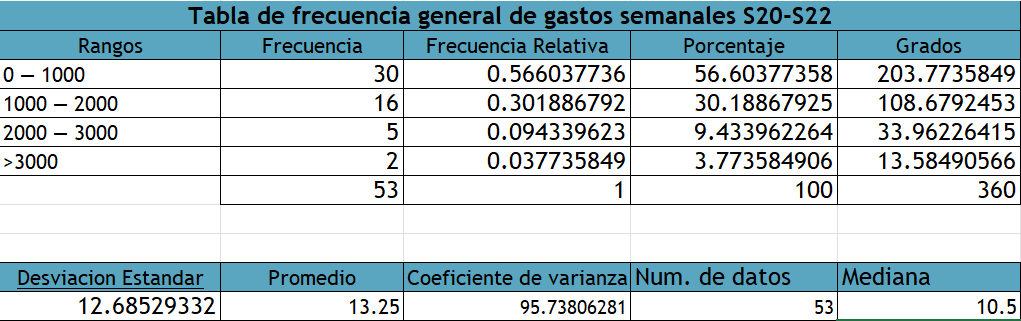
\includegraphics[width=0.9\textwidth]{images/probabilidad/Tabla de frecuencia general de gastos semanales s20-s22.PNG}
    \caption{Gastos semanales S20-S22}
\end{figure}

Como se puede observar, hay mayor frecuencia de gastos semanales en servicios (agua, transporte y entretenimiento) entre menos de \$1000 pesos entre las distintas generaciones, obtenemos un coeficiente de varianza de 95.73\% por lo que tenemos datos heterogéneos. Un 57\% de las personas que dijeron menos de \$1000 pesos  el 94\% respondió también con anterioridad que dependían económicamente y que no contaban con una beca.
\vspace{0.3cm}\\
Otra cosa más importante que decir es que el 10\% de las personas que contestaron de \$2000 a \$3000 pesos, afirmó que tienen ingresos que ayude a cubrir sus necesidades. 
\vspace{0.3cm}\\
El 67\% de los alumnos encuestados respondieron que pertenecían a la S22 y un 95\% contestó que no contaba con ninguna beca, estadísticamente el 89\% de la S22 respondió que SI dependía económicamente y que todo lo invertido en su carrera hasta ahora ha sido óptimo para un mejor aprendizaje. 
\vspace{0.3cm}\\
De todas las generaciones un 34\% pertenecía a Ingeniería Mecatrónica, destacando que el 100\% si se encontraba satisfecho con todo lo invertido en toda su carrera hasta ahora. 

En el gráfico circular nos demuestra que más de un 50\% de entre todas las generaciones (S20-S22) gastan menos de \$1,000 pesos en servicios, tomando en cuenta que este porcentaje también depende económicamente.

\begin{figure}[H]
    \centering
    \includegraphics[width=0.8 \textwidth]{images/probabilidad/gráfica general de gastos semanales s20-s22.PNG}
    \caption{Gráfica circular de gastos semanales S20-S22}
\end{figure}
Capturando una muestra más pequeña para los foráneos, los porcentajes salen más distintos para gastos semanales entre todas las generaciones, dejándonos ver que el porcentaje entre gastos de \$2000 a \$3000 y menos de \$1000 son iguales, es importante agregar que del 29\% que afirmó ser foráneo, el 94\% depende económicamente. 

\begin{figure}[H]
    \centering
    \includegraphics[width=0.8 \textwidth]{images/probabilidad/gráfica foraneos semana gastos s20-s22.PNG}
    \caption{Gráfica de gastos semanales de foráneos S20-S22}
\end{figure}

Mostrando nuestra siguiente tabla sobre cuanto dinero creen que sea necesario invertir en toda la carrera, el 57\% de los encuestados respondieron más de \$2000 y de este mismo el 90\% indicó que no contaban con una beca, no son foráneos y son de la S22. Otra cosa que destacar es que el 10\% de los que respondieron menos de \$1000 pertenecen a Ingeniería Electrónica. 

\begin{figure}[H]
    \centering
    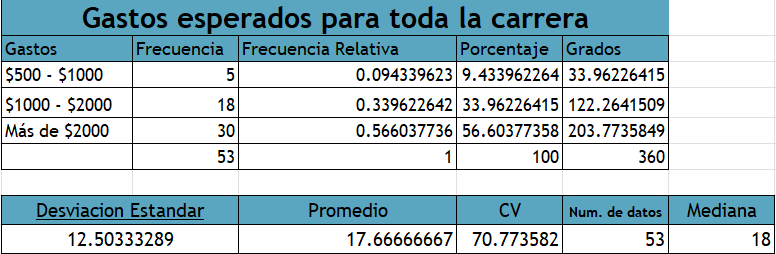
\includegraphics[width=0.9 \textwidth]{images/probabilidad/Tabla de frecuencia general de gastos esperados toda la carrera s20-s22.PNG}
    \caption{Gastos esperados a invertir S20-S22}
\end{figure}

Obtenemos datos heterogéneos con un 57\% de alumnos de S20 a S22 que piensan que en su carrera es necesario invertir más de \$2000 pesos para un buen rendimiento académico.

\begin{figure}[H]
    \centering
    \includegraphics[width=0.7 \textwidth]{images/probabilidad/gráfica de gastos esperados toda la carrera s20-s22.PNG}
    \caption{Gráfica gastos esperados a invertir S20-S22}
\end{figure}

Haciendo una comparativa de gastos que los estudiantes creen que se necesitan invertir con lo que realmente invierten desde que iniciaron la carrera, tenemos lo siguiente:

\begin{figure}[H]
    \centering
    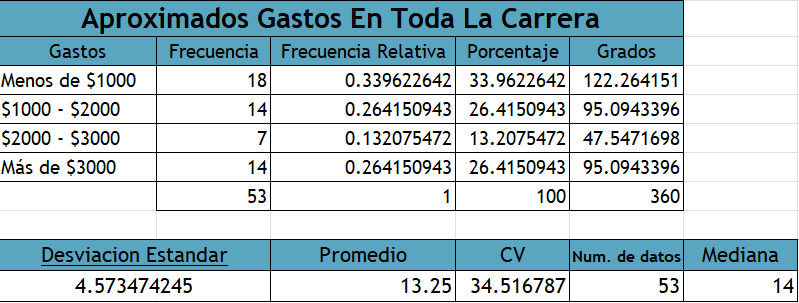
\includegraphics[width=0.9 \textwidth]{images/probabilidad/Tabla de frecuencia general de gastos aprox toda la carrera s20-s22.PNG}
    \caption{Gastos en toda la carrera a invertir S20-S22}
\end{figure}

\begin{figure}[H]
    \centering
    \includegraphics[width=0.7 \textwidth]{images/probabilidad/gráfica general de gastos aprox toda la carrera s20-s22.PNG}
    \caption{Gráfica de gastos en toda la carrera S20-S22}
\end{figure}

Obteniendo datos heterogéneos, un 34\% gasta menos de \$1000 pesos desde que inició la carrera, dentro de este porcentaje, el 94\% pertenece a la S22 y un 62\% pertenece a Ingeniería Informática, el 27\% de las personas que respondieron más de tres mil pesos afirmaron que no cuentan con una beca.

Por último también se extrajo cifrás sobre los gastos por semestre entre todas las generaciones, sorprendentemente un 42\% afirmó que invierten entre \$500 a \$1000 pesos. Independientemente del semestre, se deseaba ver un aumento o decremento de cifras entre generación, aunque la mayoría fue de la S22, se puede deducir que los gastos más altos comienzan a principios de la carrera.

\begin{figure}[H]
    \centering
    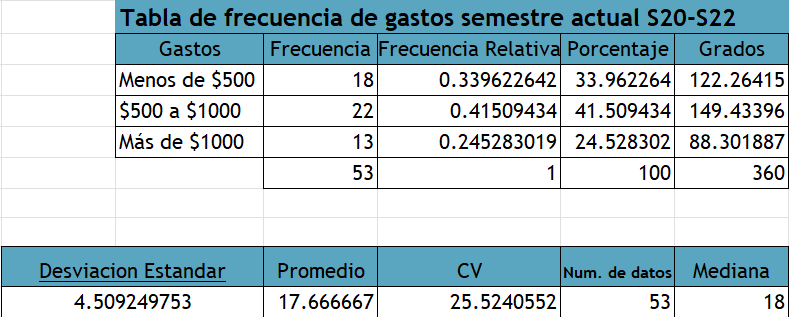
\includegraphics[width=0.7 \textwidth]{images/probabilidad/Tabla de frecuencia general de gastos sem,actual s20-s22.PNG}
    \caption{Gastos en semestre actual S20-S22}
\end{figure}

\begin{figure}[H]
    \centering
    \includegraphics[width=0.7 \textwidth]{images/probabilidad/gráfica general de gastos s actual s20-s22.PNG}
    \caption{Gráfica de gastos semestre actual S20-S22}
\end{figure}

\subsection*{Información relevante}
Un 23\% de todas las generaciones respondieron que invierten más dinero en componentes electrónicos y en computadoras, afirmando también que son los materiales que más recurso económico demandan, el 34\% afirmó gastar más en la experiencia educativa "Tecnicas de Medición".
Un 15\% comentó "computadora" como material más necesario para un mejor aprendizaje .
\vspace{0.3cm}\\
Para finalizar, se les preguntó si creen que la institución tiene el equipamiento necesario para una buena formación de carrera, el 63\% de los encuestados respondieron positivamente, el 73\% de esta cantidad no es foránea y son de la S22.Es importante aclarar que de nuestro número de datos, un 67\% es de la S22, un 11\% de la S21 y un 22\% de la S20. De las tres carreras encuestadas, un 40\% es Informática, un 33\% Mecatrónica y un 27\% Electrónica.



\newpage
\begin{center}
    \section*{Conclusión}
\end{center}
En base a todos los datos que los encuestados amablemente nos proporcionaron podemos llegar a distintivas conclusiones. La carrera que más dinero parece necesitar para materiales utilizados durante sus clases es mecatrónica, informática aunque tiene una idealización de más de \$2000 pesos, se gasta mucho menos de esa cantidad, irónicamente los electrónicos piensan que para su carrera se necesita gastar mucho menos de lo que se gasta, claro está que todo esto es tomando en cuenta los datos recabados por nuestra encuesta, a pesar de no llegar a una cifrá de respuestas más demantante entre las otras generaciones, la S22 nos da una idea de esas expectativas de carrera que se tienen y sin embargo por situaciones económicas y no mucho apoyo de la institución o terceros, se termina bajando todo ese presupuesto que se supone los propios alumnos necesitan para un mejor aprendizaje. 
\vspace{0.3cm}\\
Retomando las observaciones de porcentajes, los de ingeniería mecatrónica requieren componentes eléctricos y muchos de estos no son son realmente costosos si se requiere tener un flujo más o menos continuo de piezas nuevas para armar proyectos o reemplazar los que se hayan roto, en informática las grandes sumas de dinero son comúnmente por la necesidad de adquirir equipos informáticos (laptops) para poder continuar y sistematizar mejor sus prácticas, al final del día muchos se conforman con este material y dejan mucho de lado otros materiales que comparten mecatrónica y electrónica, que al final parece que estos últimos realmente no necesitan tantos materiales. 
\vspace{0.3cm}\\
Aún con las diferentes razones y grandes cifras por las cuales diferentes alumnos de diferentes carreras puedan o no conseguir el capital necesario para sus clases, todos parecen coincidir en que la escuela debería tener más equipamiento para cumplir con las necesidades de los estudiantes, contribuir a mejores laboratorios para reforzar habilidades necesarias y con la seguridad de hacerlo sin peligro. Tomando en cuenta que la mayoría de nuestros encuestados son dependientes de ayuda externa (de sus padres o un tutor) para tener ingresos suficientes que ayudan a mantener sus actividades normales en la facultad, estos tienden a oscilar entre valores de \$0 a \$1000 pesos a la semana contando los servicios ya mencionados anteriormente, estas cifras tienen sentido para alguien que no debe generar ingresos por cuenta propia, sin embargo, por porcentajes nos podemos dar cuenta que muchos estudiantes no se sentían seguros con sus ingresos y con lo que se supone deberían gastar, esto tiene cierto contraste en  el caso de los foráneos, de todo lo que gastan en la semana, no pueden invertir mucho más de sus chances, y más que eso, piensan que se debe gastar mucho más de lo que generan, debemos tomar en cuenta que los estudiantes esperan gastar mucho más para los siguientes semestres. 
\vspace{0.3cm}\\
Esto no sería una gran problemática si no fuera por el hecho de que el 92\% de los encuestados no tienen una beca, si bien podemos decir que menos del 30\% son foráneos, ese pequeño porcentaje muestra falta de apoyo respecto al uso de materiales y otros bienes necesarios. 
\vspace{0.3cm}\\
Podemos concluir que los alumnos no se sienten con el dinero suficiente o con las herramientas necesarias para el hábil y efectivo desarrollo de sus habilidades, y si la escuela no tiene la capacidad de proporcionar dichos materiales necesarios, la siguiente mejor opción sería mejorar los planes de becas para un estudiante que si lo necesita por cualquier pieza, elemento, programa o licencia para poder continuar con sus actividades dentro del plantel, la institución puede apoyarlo y así seguramente todos los estudiantes tengan la oportunidad de conseguir terminar su carrera con los conocimientos necesarios adquiridos durante la práctica en laboratorios bien equipados y un buen apoyo docente, así asegurando el futuro de los jóvenes y de todos.


\newpage
\begin{center}
    \section*{Bibliografía}
\end{center}



    


\end{sloppypar}
\end{document}